\section{Resultater}
\label{SkaleringseksperimentResultater}
%
Testen blev udført på otte testpersoner; tre kvinder og fem mænd, med et aldersspænd fra 21 år til 34 år (gennemsnit: 24.6 år). Testpersonerne er alle studerende på Aalborg Universitet fordelt på følgende studieretninger: Jura, Kemi-Teknologi, Fysisk og Biologi.\blankline
%
På \autoref{fig:RaaDataTestpersoner} fremgår de otte testpersoners individuelle vurderinger af, hvor indbydende robotten perciperes afhængigt af hovedposition.  
%
\begin{figure}[H]
\centering
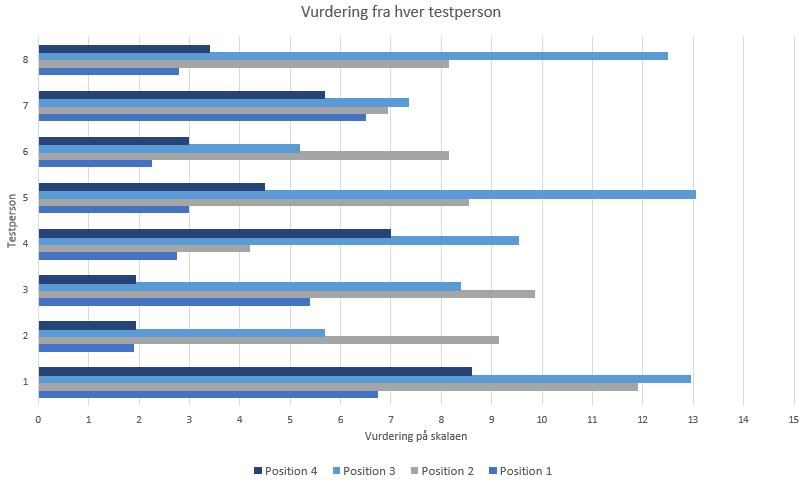
\includegraphics[width = \textwidth]{Figure/RaaDataTestpersoner.PNG} 
\caption{Rådata fra hver testperson. X-aksen er defineret ud fra den definerede skala-længde, hvorfor x-værdierne afspejler hvor indbydende testpersonen perciperer robotten. Testpersonerne er angivet på y-aksen.}
\label{fig:RaaDataTestpersoner}
\end{figure}
\noindent
%
\autoref{fig:RaaDataPositioner} er en sorting af data, som afspejler hvor indbydende hver testperson perciperer den specifikke hovedposition. 
%
\begin{figure}[H]
\centering
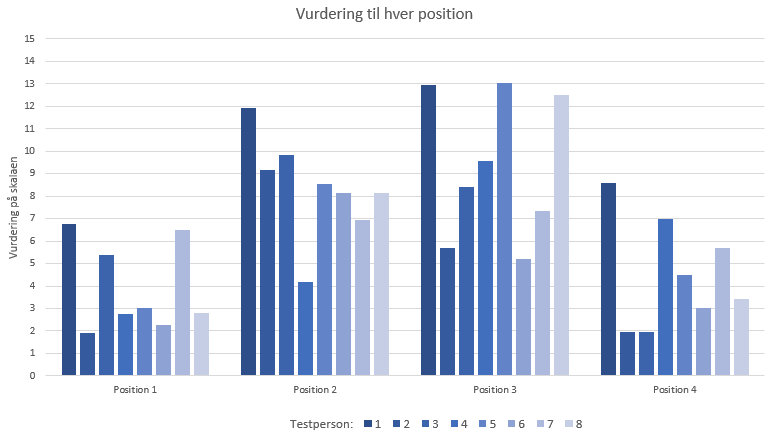
\includegraphics[width = \textwidth]{Figure/RaaDataPositioner.PNG} 
\caption{Rådata sorteret efter de fire hovedpositioner, repræsenteret på x-aksen, hvor y-aksen gengiver hvor indbydende hver testperson perciperer robotten afhængigt af hovedposition.}
\label{fig:RaaDataPositioner}
\end{figure}
\noindent
%
Med udgangspunkt i \autoref{fig:RaaDataPositioner} tyder det på, at både position 2 og position 3 perciperes som værende mere indbydende end både position 1 og position 4.\blankline
%
For at besvare hypoteserne, opstillet i \fullref{SkaleringseksperimentHypotese}, vil der i følgende afsnit udføres statistiske analyser.   

